% !TeX spellcheck = it_IT
\documentclass{article}
\usepackage[utf8]{inputenc}
\inputencoding{utf8}
\usepackage[T1]{fontenc}
\usepackage{fancyhdr} % Required for custom headers
\usepackage{lastpage} % Required to determine the last page for the footer
\usepackage{extramarks} % Required for headers and footers
\usepackage[usenames,dvipsnames]{color} % Required for custom colors
\usepackage{graphicx} % Required to insert images
\usepackage{listings} % Required for insertion of code
\usepackage{courier} % Required for the courier font
\usepackage{lipsum} % Used for inserting dummy 'Lorem ipsum' text into the template
\usepackage{hyperref}
\usepackage{multirow}
\usepackage{tabularx}
\usepackage{longtable}
\usepackage{listings}
\usepackage{subfigure}
\usepackage{afterpage}
\usepackage{amsmath,amssymb}            
\usepackage{fancyhdr}
\usepackage{graphicx}
\usepackage{amsthm}
\usepackage[scriptsize]{caption} 
\hyphenation{a-gen-tiz-za-zio-ne}
% Margins
\topmargin=-0.45in
\evensidemargin=0in
\oddsidemargin=0in
\textwidth=6.5in
\textheight=9.0in
\headsep=0.25in

\linespread{1.1} % Line spacing

\lstset{
	numbers=left,
	stepnumber=5,    
	firstnumber=1,
	numberfirstline=true
}

% Set up the header and footer
\pagestyle{fancy}
\lhead{\hmwkAuthorName} % Top left header
\chead{\hmwkClass\ (\hmwkClassInstructor\ \hmwkClassTime): \hmwkTitle} % Top center head
\rhead{\firstxmark} % Top right header
\lfoot{\lastxmark} % Bottom left footer
\cfoot{} % Bottom center footer
\rfoot{Page\ \thepage\ of\ \protect\pageref{LastPage}} % Bottom right footer
\renewcommand\headrulewidth{0.4pt} % Size of the header rule
\renewcommand\footrulewidth{0.4pt} % Size of the footer rule

\setlength\parindent{0pt} % Removes all indentation from paragraphs

\usepackage{listings}
\usepackage{color}
\usepackage{graphicx}
\usepackage{mathrsfs}
\usepackage{framed}
\usepackage{amssymb}
\usepackage[figuresright]{rotating}
\usepackage{comment}
\usepackage{listings}
\usepackage{xcolor}
\usepackage{amsmath}
\usepackage{algpseudocode}
\usepackage{algorithm}
\usepackage{flushend}
\usepackage{times}
\usepackage{url}
\usepackage{comment}
\usepackage{paralist}
\usepackage[multiple]{footmisc}
\usepackage{amsthm}
\usepackage{multicol}


\definecolor{dkgreen}{rgb}{0,0.6,0}
\definecolor{gray}{rgb}{0.5,0.5,0.5}
\definecolor{mauve}{rgb}{0.58,0,0.82}

\lstset{frame=tb,
	language=Java,
	aboveskip=3mm,
	belowskip=3mm,
	showstringspaces=false,
	columns=flexible,
	basicstyle={\small\ttfamily},
	numbers=none,
	numberstyle=\tiny\color{gray},
	keywordstyle=\color{blue},
	commentstyle=\color{dkgreen},
	stringstyle=\color{mauve},
	breaklines=true,
	breakatwhitespace=true
	tabsize=3,
	literate={à}{{\'a}}1
	{è}{{\'e}}1
	{ì}{{\'u}}1
	{ò}{{\'o}}1
	{ù}{{\'u}}1
}
%----------------------------------------------------------------------------------------
%	DOCUMENT STRUCTURE COMMANDS
%	Skip this unless you know what you're doing
%----------------------------------------------------------------------------------------

% Header and footer for when a page split occurs within a problem environment
\newcommand{\enterProblemHeader}[1]{
\nobreak\extramarks{#1}{#1 continued on next page\ldots}\nobreak
\nobreak\extramarks{#1 (continued)}{#1 continued on next page\ldots}\nobreak
}

% Header and footer for when a page split occurs between problem environments
\newcommand{\exitProblemHeader}[1]{
\nobreak\extramarks{#1 (continued)}{#1 continued on next page\ldots}\nobreak
\nobreak\extramarks{#1}{}\nobreak
}




\newcommand{\hmwkTitle}{03 - Ereditariet\`a e Conversioni} % Assignment title
\newcommand{\hmwkDueDate}{Martedì,\ Marzo 22,\ 2016} % Due date
\newcommand{\hmwkClass}{Ingegneria del Software 1} % Course/class
\newcommand{\hmwkClassTime}{} % Class/lecture time
\newcommand{\hmwkClassInstructor}{Claudio Menghi, Alessandro Rizzi} % Teacher/lecturer
\newcommand{\hmwkAuthorName}{} % Your name


\author{\textbf{\hmwkAuthorName}}
\date{} % Insert date here if you want it to appear below your name
\newcounter{EsercizioCounter}
 \setcounter{EsercizioCounter}{1}


\newcommand{\Esercizio}[1]{
%\setlength{\fboxsep}{2pt}
\fbox{
   
  \parbox[t][]{\textwidth}{
   \vspace{2ex}
   \textbf{Esercizio \arabic{EsercizioCounter}}: #1
    \vspace{2ex}
    \refstepcounter{EsercizioCounter}
  }
}
}


%----------------------------------------------------------------------------------------

\begin{document}

\maketitle

%----------------------------------------------------------------------------------------
%	TABLE OF CONTENTS
%----------------------------------------------------------------------------------------

%\setcounter{tocdepth}{1} % Uncomment this line if you don't want subsections listed in the ToC

\newpage
\tableofcontents
\newpage



\section{Introduction}


\subsection{Polimorfismo}
Attraverso il \emph{polimorfismo} \`e possibile utilizzare un oggetto di tipo \texttt{S} al posto di un oggetto di tipo \texttt{T}, se \texttt{S} \`e un sottotipo di \texttt{T}.\\
Il tipo  \emph{statico} \`e usato nella dichiarazione della variabile e determina l'insieme dei metodi che possono essere invocati, mentre il tipo \emph{dinamico} \`e  quello realmente istanziato e referenziato in memoria e stabilisce quale sar\`a l'implementazione usata.

Per esempio, data la gerarchia presentata in Figura~\ref{Fig:gerarchy1}, una variabile di tipo (statico) \texttt{Animale} pu\`o essere sostituita da una variabile di tipo (dinamico) \texttt{Cane} o \texttt{Gatto}.

\begin{figure}[h!]
  \centering
    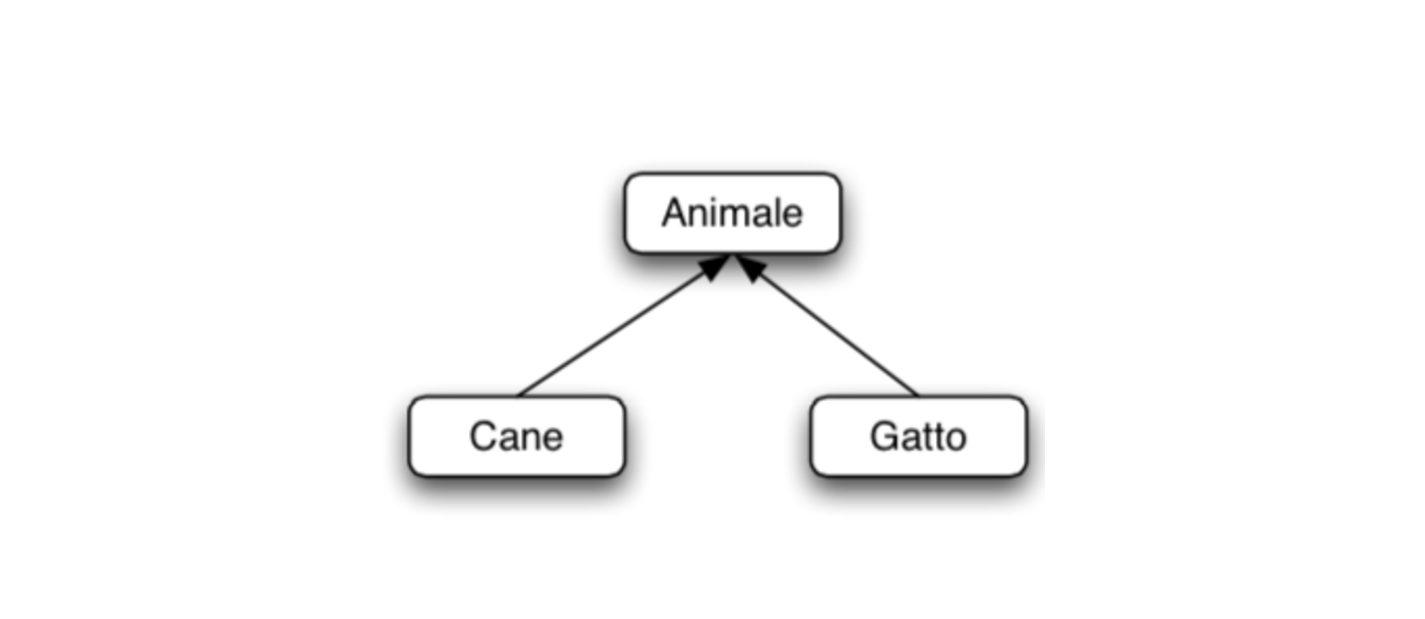
\includegraphics[width=0.5\textwidth]{gerarchia.pdf}
      \caption{Un semplice esempio di gerarchia.}
      \label{Fig:gerarchy1}
\end{figure}
\begin{lstlisting}
Animale a=new Cane();
Cane c=new Animale();
\end{lstlisting}
La prima istruzione \`e corretta: \`e possibile assegnare a una variabile di tipo (statico) \texttt{Animale} una variabile di tipo \texttt{Cane}.
La seconda istruzione non \`e corretta: non \`e possibile assegnare a una variabile di tipo (statico) \texttt{Cane} una variabile di un sopra-tipo \texttt{Animale}, il compilatore mostra l'errore \emph{type mismatch: cannot convert from Animale to Cane}.

Consideriamo questo semplice esempio:

\begin{lstlisting}
public class Animale {
    public Animale gioca(Animale altroAnimale){
        System.out.println("Animale: gioca"); 
        return altroAnimale;
    }
}
public class Cane extends Animale { 
}
public class Main {
    public static void main(String[] args) { 
        Animale b=new Cane();
        Animale a=new Cane();
        a.gioca(b);
    } 
}
\end{lstlisting}

A \emph{compile-time} viene controllato che l'invocazione del metodo \texttt{gioca} sia lecita: \`e possibile invocare il metodo gioca su una variabile di tipo statico \texttt{Animale} passando come parametro una variabile di tipo statico \texttt{Animale}. Nel caso specifico \`e lecito chiamare il metodo gioca su una variabile \texttt{a} di tipo (statico) \texttt{Animale}, passando come parametro la variabile \texttt{b} di tipo (statico) \texttt{Animale}. La signature prescelta del metodo \`e \texttt{public Animale gioca(Animale altroAnimale)}. A \emph{run-time} la variabile \texttt{a} \`e di tipo \texttt{Cane}, per cui viene chiamato il metodo \texttt{Animale gioca(Animale altroAnimale)} della classe \texttt{Cane} che \`e ereditato dalla classe \texttt{Animale}. Il metodo stampa ``\textit{Animale: gioca}".

Consideriamo ora il seguente:
\begin{lstlisting}
public class Animale {
    public Animale gioca(Animale altroAnimale){
        System.out.println("Animale: gioca"); return altroAnimale;
    }
}
public class Cane extends Animale { 
}
public class Main {
    public static void main(String[] args) { 
        Cane b=new Cane();
        Animale a=new Cane();
        a.gioca(b);
    } 
}
\end{lstlisting}

A \emph{compile-time} viene controllato che l'invocazione del metodo \texttt{gioca} sia lecita: \`e possibile invocare il metodo gioca su una variabile di tipo statico \texttt{Animale} passando come parametro una variabile di tipo statico \texttt{Cane}. Nel caso specifico \`e lecito chiamare il metodo gioca (con signature \texttt{public Animale gioca(Animale altroAnimale)}) su una variabile \texttt{a} di tipo (statico) \texttt{Animale}, passando come parametro la variabile \texttt{b} di tipo (statico) \texttt{Cane} visto che \texttt{Cane} \`e sottotipo di \texttt{Animale}. A \emph{run-time} la variabile \texttt{a} \`e di tipo \texttt{Cane}, per cui viene chiamato il metodo \texttt{Animale gioca(Animale altroAnimale)} della classe \texttt{Cane} che \`e ereditato dalla classe \texttt{Animale}. Il metodo stampa ``\textit{Animale: gioca}".

\begin{lstlisting}
public class Animale {
    public Animale gioca(Animale altroAnimale){
        System.out.println("Animale:␣gioca"); 
        return altroAnimale;
    }
}
public class Cane extends Animale {
    public Animale gioca(Cane altroAnimale){ 
        System.out.println("Cane:␣gioca"); 
        return altroAnimale;
    }
}
public class Main {
    public static void main(String[] args) { 
        Cane b=new Cane();
        Animale a=new Cane();
        a.gioca(b);
   } 
}
\end{lstlisting}
A \emph{compile-time} viene controllato che l'invocazione del metodo \texttt{gioca} sia lecita: \`e possibile invocare il metodo gioca su una variabile di tipo statico \texttt{Animale} passando come parametro una variabile di tipo statico \texttt{Cane}. Nel caso specifico \`e lecito chiamare il metodo gioca (con signature \texttt{public Animale gioca(Animale altroAnimale)}) su una variabile \texttt{a} di tipo (statico) \texttt{Animale}, passando come parametro la variabile \texttt{b} di tipo (statico) \texttt{Cane} visto che \texttt{Cane} \`e sottotipo di \texttt{Animale}. A \emph{run-time} la variabile \texttt{a} \`e di tipo \texttt{Cane}, viene chiamato il metodo \texttt{Animale gioca(Animale altroAnimale)} scelto durante la fase di compilazione su una variabile di tipo dinamico \texttt{Cane}, per cui viene chiamato il metodo \texttt{Animale gioca(Animale altroAnimale)} della classe cane che \`e ereditato dalla classe \texttt{Animale}. Il metodo stampa ``\textit{Animale: gioca}".

\begin{lstlisting}
public class Animale {
    public Animale gioca(Animale altroAnimale){
        System.out.println("Animale:␣gioca");
        return altroAnimale; 
    }
}
public class Cane extends Animale { 
    public Animale gioca(Cane altroAnimale){
        System.out.println("Cane:␣gioca");
        return altroAnimale; 
    }
}
public class Main {
    public static void main(String[] args) {
        Cane b=new Cane(); 
        Animale a=new Cane(); 
        b.gioca(a);
   } 
}
\end{lstlisting}
A \emph{compile-time} viene controllato che l'invocazione del metodo \texttt{gioca} sia lecita: \`e possibile invocare il metodo gioca su una variabile di tipo statico \texttt{Cane} passando come parametro una variabile di tipo statico \texttt{Animale}. Nel caso specifico \`e lecito chiamare il metodo gioca su una variabile \texttt{b} di tipo (statico) \texttt{Cane}, passando come parametro la variabile \texttt{a} di tipo (statico) \texttt{Animale}.
La signature prescelta \`e \texttt{public Animale gioca(Animale altroAnimale)}. \\
A \emph{run-time} la variabile \texttt{b} \`e di tipo \texttt{Cane}, viene chiamato il metodo \texttt{Animale gioca(Animale} \texttt{altroAnimale)} scelto durante la fase di compilazione su una variabile di tipo dinamico \texttt{Cane}, per cui viene chiamato il metodo \texttt{Animale gioca(Animale altroAnimale)} della classe \texttt{Cane} che \`e ereditato dalla classe \texttt{Animale}. Il metodo stampa ``\textit{Animale: gioca}".

\begin{lstlisting}
public class Animale {
    public Animale gioca(Animale altroAnimale){
        System.out.println("Animale:␣gioca"); 
        return altroAnimale;
    }
}
public class Cane extends Animale {
    public Animale gioca(Cane altroAnimale){ 
        System.out.println("Cane:␣gioca"); 
        return altroAnimale;
    }
}
public class Main {
    public static void main(String[] args) { 
        Cane b=new Cane();
        Animale a=new Cane();
        b.gioca(b);
    } 
}
\end{lstlisting}
A \emph{compile-time} viene controllato che l'invocazione del metodo \texttt{gioca} sia lecita: \`e possibile invocare il metodo gioca su una variabile di tipo statico \texttt{Cane} passando come parametro una variabile di tipo statico \texttt{Cane}. Nel caso specifico \`e lecito chiamare il metodo gioca su una variabile \texttt{b} di tipo (statico) \texttt{Cane}, passando come parametro la variabile \texttt{a} di tipo (statico) \texttt{Cane}.
La signature prescelta \`e \texttt{public Animale gioca(Cane altroAnimale)}. \\
A \emph{run-time} la variabile \texttt{b} \`e di tipo \texttt{Cane}, viene chiamato il metodo \texttt{Animale gioca(Cane} \texttt{altroAnimale)} scelto durante la fase di compilazione su una variabile di tipo dinamico \texttt{Cane}, per cui viene chiamato il metodo \texttt{Animale gioca(Animale altroAnimale)} della classe \texttt{Cane} che \`e ereditato dalla classe \texttt{Animale}. Il metodo stampa ``\textit{Cane: gioca}".

\subsection{Interfacce}
Partiamo dalla struttura definita in Figura~\ref{Fig:gerarchy2}. Come \`e possibile estendere la gerarchia al fine di supportare gli animali che possono volare?

\begin{figure}[h!]
  \centering
    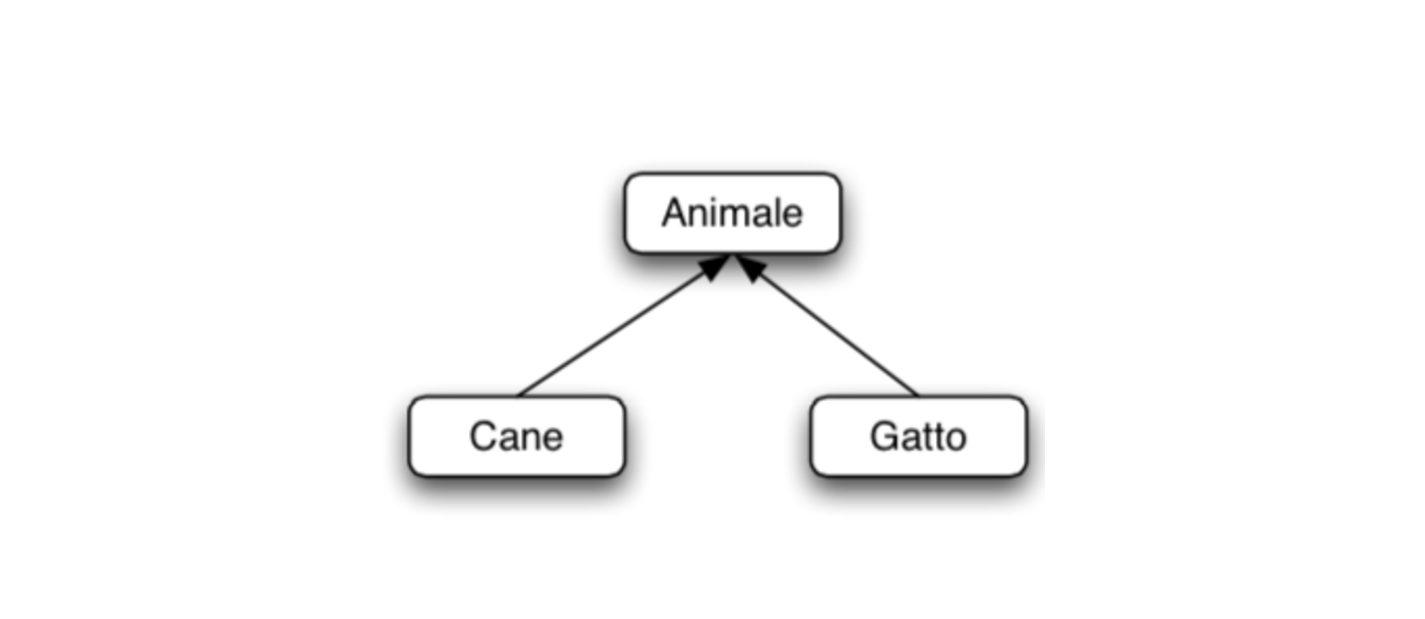
\includegraphics[width=0.5\textwidth]{gerarchia.pdf}
      \caption{Un semplice esempio di gerarchia.}
      \label{Fig:gerarchy2}
\end{figure}

La prima soluzione consiste nell'introdurre una nuova classe \texttt{Volatile} che contiene gli animali che possono volare. La classe \texttt{Gufo} contiene uno specifico tipo di volatili. \\

\begin{figure}[h!]
  \centering
    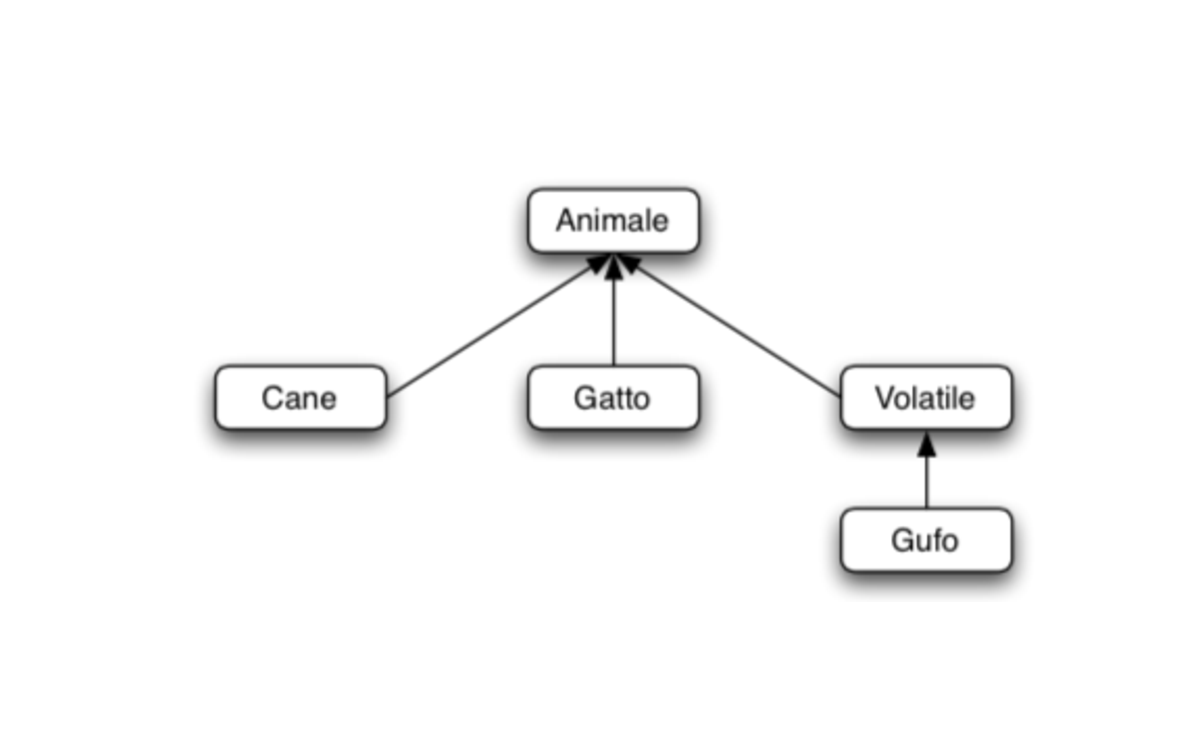
\includegraphics[width=0.5\textwidth]{gerarchia2.pdf}
      \caption{Un esempio di gerarchia che supporta la descrizione di animali che possono volare.}
      \label{Fig:gerarchy3}
\end{figure}

Come potremmo modificare la nostra gerarchia al fine di supportare gli animali che possono nuotare?
Seguendo l'idea descritta in precedenza potremmo proporre la gerarchia descritta in Figura~\ref{Fig:gerarchy4}. Tuttavia, l'introduzione della classe \texttt{Acquatico} non \`e sufficiente a modificare la gerarchia come desiderato. Infatti, l'introduzione di questa classe ci permette di specificare che un \texttt{Pesce} \`e un animale acquatico, ma non ci permette di dire che un \texttt{Anatra} \`e un animale acquatico ma allo stesso tempo \`e un volatile. Per fare questo \`e necessario introdurre la classe \texttt{VolatileAcquatico} capace di rappresentare l'insieme dei volatili che sono anche animali acquatici.
\begin{figure}[h!]
  \centering
    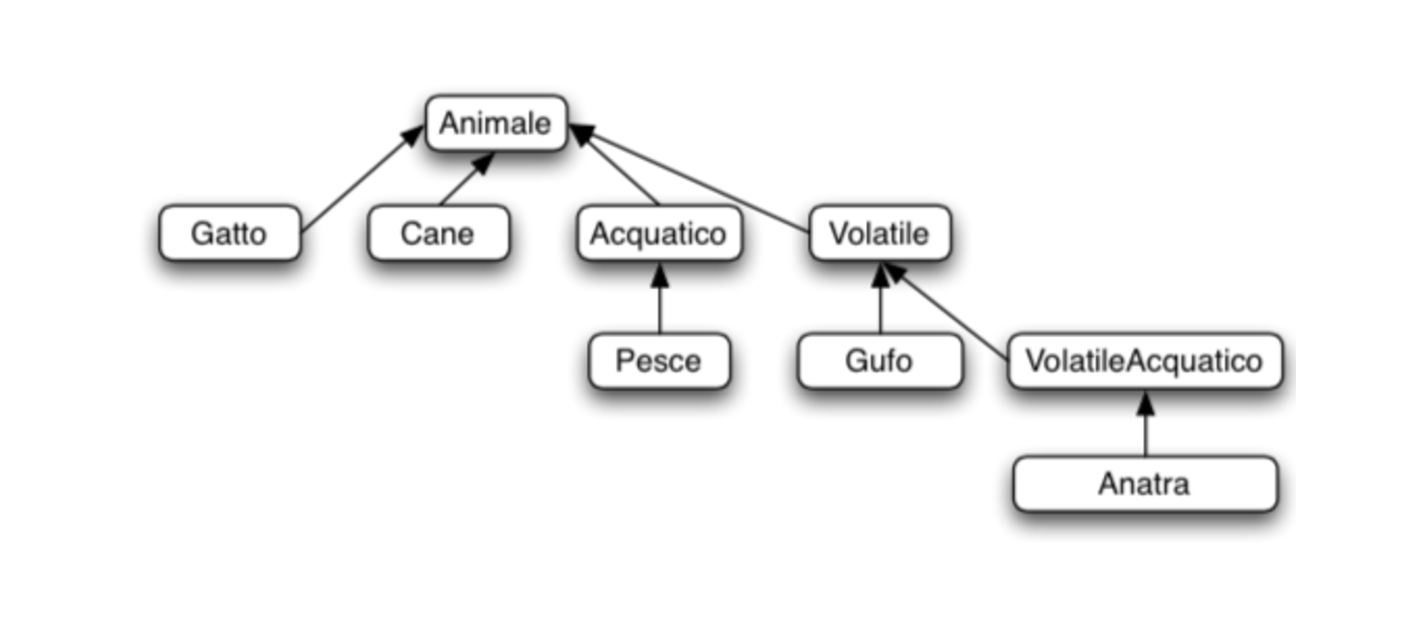
\includegraphics[width=0.5\textwidth]{gerarchia3.pdf}
      \caption{Un esempio di gerarchia che supporta la descrizione di animali che possono volare.}
      \label{Fig:gerarchy4}
\end{figure}
La modifica effettuata rende la gerarchia \emph{molto complicata}. Inoltre, \`e evidente come una piccola modifica (per esempio una nuova  propriet\`a) comporta modifiche rilevanti alla gerarchia. Infine, la gerarchia contiene un \textbf{grave} problema concettuale: non dice che \texttt{Pesce} e \texttt{Anatra} appartengono alla medesima categoria ``Acquatico".

Un modo per ottenere questa propriet\`a \`e quella di utilizzare l'ereditariet\`a multipla. In questo caso i concetti diversi risultano separati e ciascuna classe pu\`o ereditare quelli che servono. Java non supporta l'ereditariet\`a multipla. Questa astrazione viene ottenuta per mezzo delle \emph{interfacce}.

\begin{itemize}
\item Una \emph{classe} ci dice che un oggetto \`e qualche cosa
\item Un \emph{interfaccia} rappresenta un comportamento che la classe fornisce
\end{itemize}

Figura~\ref{Fig:gerarchy4} presenta una gerarchia che risolve il problema precedente: \`e una gerarchia pi\`u semplice e permette di descrivere tutti i concetti che ci servono.
\begin{figure}[h!]
  \centering
    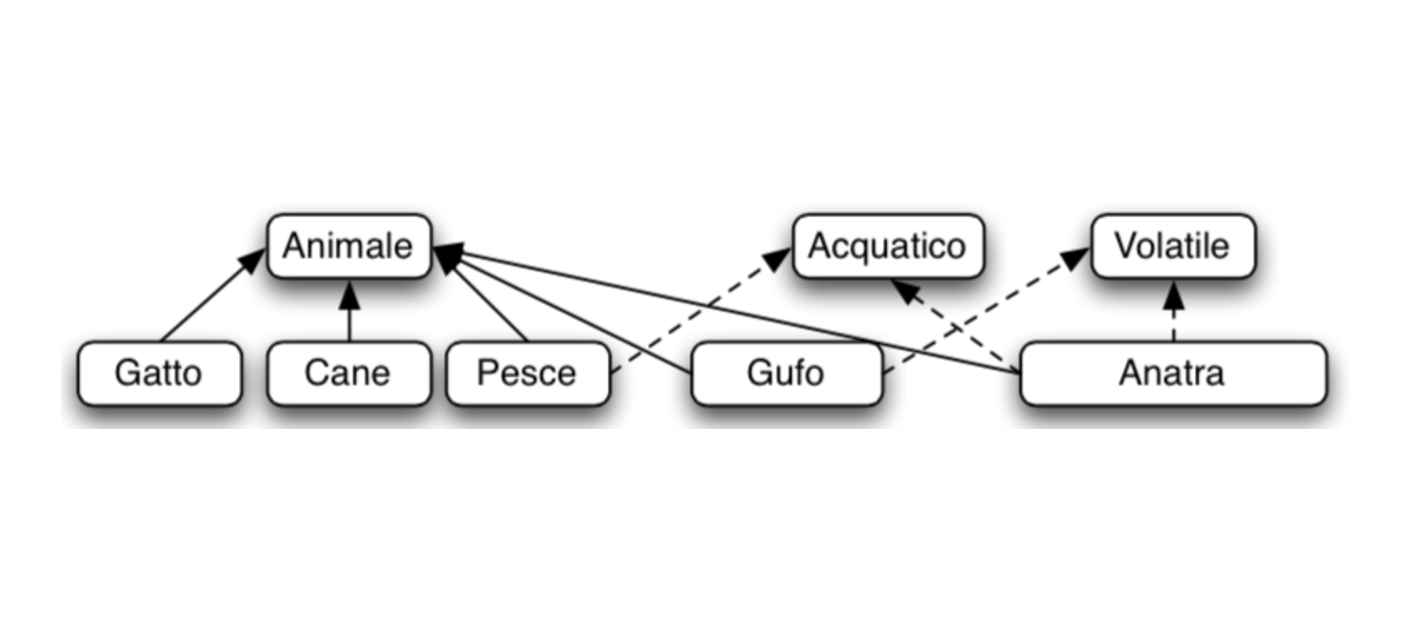
\includegraphics[width=0.5\textwidth]{gerarchia4.pdf}
      \caption{Un esempio di gerarchia che risolve il problema precedente.}
      \label{Fig:gerarchy4}
\end{figure}

Una bozza di implementazione \`e presentata in seguito.
\begin{lstlisting}[language=Java,escapechar=|]
public class Anatra extends Animale implements Volatile, Acquatico { 
    // Ha tutto ciò che aveva la classe Animale
    // Deve implementare i metodi definiti in Volatile e in Acquatico 
    @Override
    public void vola(){ ... }
    @Override
    public void nuota(){ ... } 
}
\end{lstlisting}
Le interfacce possono essere utilizzate come tipo (statico) di riferimento. Come tipo statico l'interfaccia espone tutti i metodi che definisce.
L'implementazione utilizzata dipende dal \emph{tipo dinamico} della classe (Binding dinamico). Per gli assegnamenti dobbiamo considerare le relazioni di tipo/sotto-tipo.



\subsection{HashCode and Equals}
I metodi \texttt{hashCode()} e \texttt{equals()} sono molto utilizzati nella programmazione a oggetti. In particolare:
\begin{itemize}
\item \texttt{hashCode()} la funzione hash \`e una funzione non iniettiva (e quindi non invertibile) che mappa una oggetto in una intero in genere \`e opportuno che l'algoritmo di hashing soddisfi le seguenti caratteristiche
\begin{itemize}
\item quando \`e invocato pi\`u di una volta sullo stesso oggetto deve ritornare lo stesso intero (questo intero potrebbe essere diverso in esecuzioni diverse dell'applicazione, l'importante \`e che all'interno di un esecuzione sia sempre lo stesso)
\item se due oggetti sono uguali con riferimento al metodo \texttt{equals} allora  il metodo \texttt{hashCode} deve ritornare lo stesso intero
\item non \`e richiesto che due oggetti non uguali in termini del metodo \texttt{equals} siano associati due \texttt{hashCode} diversi. Tuttavia, il programmatore deve sapere che produrre interi differenti pu\`o migliorare le performances (per esempio nel caso delle \texttt{HashMap}).
\end{itemize}
\item \texttt{equals()} specifica quando un oggetto \`e uguale all'oggetto corrente. Il metodo \texttt{equals} implementa una relazione di equivalenza su degli elementi non nulli. La relazione deve essere
\begin{itemize}
\item \emph{riflessiva} per ogni reference \texttt{x} non nullo \texttt{x.equals(x)} ritorna \texttt{true}
\item \emph{symmetrica} per ogni references \texttt{x} e \texttt{y} non nulli \texttt{x.equals(y)} deve ritornare \texttt{true} se e solo se \texttt{y.equals(x)} ritorna \texttt{true}
\item \emph{transitiva} per ogni \texttt{x}, \texttt{y}, \texttt{z} non nulli se \texttt{x.equals(y)} ritorna true, e \texttt{y.equals(z)} ritorna true allora \texttt{x.equals(z)} deve ritornare \texttt{true}.
\item \emph{consistente}: per ogni \texttt{x} e \texttt{y} non nulli, invocazioni multiple di \texttt{x.equals(y)} devono ritornare consistentemente \texttt{true} o consistentemente \texttt{false} se nessuna informazione utilizzata nel metodo \texttt{equals} \`e modificato.
\item per ogni reference \texttt{x} non nullo, \texttt{x.equals(null)} dovrebbe ritornare \texttt{false}
\end{itemize}
\end{itemize}

\subsection{Auto-boxing e auto-unboxing}
Dalla versione \emph{1.5} Java fornisce le funzionalit\`a di Auto-boxing e Auto-unboxing.
\begin{itemize}
\item \emph{Auto-boxing}: conversione automatica che il compilatore di Java effettua tra tipi primitivi e le corrispondenti classi di wrapper.
Per esempio \`e possibile convertire automaticamente un \texttt{int} in un \texttt{Integer} un \texttt{double} in un \texttt{Double} etc.\\
\item \emph{Auto-unboxing}: permette di convertire un tipo reference nel corrispondente tipo primitivo, per esempio di convertire un \texttt{Integer} in un intero.
\end{itemize}
Considera il seguente codice:
\begin{lstlisting}[language=Java,escapechar=|]
List<Integer> li = new ArrayList<Integer>();
for (int i = 1; i < 50; i += 2)
    li.add(i);
\end{lstlisting}
\`E possibile aggiungere a una lista di tipo \texttt{Integer} \texttt{li} un elemento \texttt{i} di tipo \texttt{int}, sebbene \texttt{i} sia di un tipo primitivo mentre gli elementi in \texttt{li} siano di tipo reference. Questo perch\`e il compilatore crea degli oggetti di tipo \texttt{Integer} partendo dalla variabile \texttt{i}.

\subsection{Casting}
Abbiamo visto che il tipo dinamico di un oggetto dipende dal tipo della classe utilizzata per istanziarlo. Per esempio, se scriviamo:
\begin{lstlisting}[language=Java,escapechar=|]
MountainBike myBike = new MountainBike();
\end{lstlisting}
l'oggetto \texttt{myBike} sar\`a di tipo \texttt{MountainBike}, dove  \texttt{MountainBike} \`e un discendente della classe \texttt{Bicycle} che a sua volta discende da \texttt{Object}. Di conseguenza, una \texttt{MountainBike} \`e sia una \texttt{Bicycle} sia un \texttt{Object} e pu\`o essere sostituito a un oggetto di tipo \texttt{Bicycle} o \texttt{Object}.

Il contrario non \`e necessariamente vero: una \texttt{Bicycle} potrebbe essere una \texttt{MountainBike} ma non necessariamente. In maniera analoga un oggetto potrebbe essere una \texttt{Bicycle} o una \texttt{MountainBike}, ma non necessariamente. Il casting degli oggetti permette di utilizzare un oggetto di un tipo al posto di un oggetto di un altro tipo. Per esempio, se scriviamo 

\begin{lstlisting}[language=Java,escapechar=|]
Object obj = new MountainBike();
\end{lstlisting}
l'oggetto \texttt{obj} \`e sia un oggetto che una \texttt{MountainBike} (se non riassegnato). Questo viene chiamato \emph{casting implicito}.

A questo punto, se scriviamo: 
\begin{lstlisting}[language=Java,escapechar=|]
MountainBike myBike = obj;
\end{lstlisting}
otteniamo un errore a \emph{compile-time} perch\`e il compilatore non \`e consapevole che \texttt{obj} \`e di classe \texttt{MountainBike}. Tuttavia, possiamo dire al compilatore di convertire \texttt{obj} in un oggetto di tipo \texttt{MountainBike} (``promettiamo al compilatore che a run-time \texttt{obj} sar\`a di tipo \texttt{MountainBike}").

\begin{lstlisting}[language=Java,escapechar=|]
MountainBike myBike = (MountainBike)obj;
\end{lstlisting}
Se a run-time \texttt{obj} non \`e di tipo \texttt{MountainBike} viene generata una opportuna eccezione.

\section{Esercizi}


\subsection{Polimorfismo e binding dinamico}
\subsection{Esercizio 6: Tipo statico e tipo dinamico}
Dire cosa stampa il seguente programma 
\begin{lstlisting}[language=Java,escapechar=|]
public static void main(String[] args) {
		ClassA a1, a2;
		ClassB b1;
		ClassC c1;

		a1 = new ClassB();
		b1 = new ClassB();
		c1 = new ClassC();
		a2 = new ClassC();

		/*
		 * b1 e' di classe ClassB, viene chiesto di invocare il metodo stampa su
		 * un parametro b1 di tipo statico ClassB. A compile scelgo la signature
		 * "compatibile" e piu' "vicina", considerando i tipi statici delle
		 * variabili. In particolare in questo caso la signature scelta e'
		 * public void stampa(ClassB p).
		 * 
		 * A run time b1 e' di classe classB e e il parametro p, che equivale a
		 * B1 e' anch'esso di classe ClassB per cui viene chiamato il metodo
		 * public void stampa(ClassB p) di class B (stampa BBB)
		 */
		b1.stampa(b1);
		/*
		 * a1 e' di classe ClassA, viene chiesto di invocare il metodo stampa su
		 * un parametro b1 di tipo statico ClassB. A compile scelgo la signature
		 * "compatibile" e piu' "vicina", considerando i tipi statici delle
		 * variabili. In particolare in questo caso la signature scelta e'
		 * public void stampa(ClassA p) della classe ClassA.
		 * 
		 * A run-time a1 e' di classe ClassB. Per questo partendo da classB e
		 * risalendo nella gerarchia di raffinamento cerco un metodo che matchi
		 * la signature public void stampa(ClassA p). In questo caso il metodo
		 * e' gia' presente in ClassB. Quindi viene invocato il metodo public
		 * void stampa(ClassA p) della classe ClassB (Stampa AAA/BBB)
		 */
		a1.stampa(b1);

		/*
		 * b1 e' di classe ClassB, viene chiesto di invocare il metodo stampa su
		 * un parametro c1 di tipo statico ClassC. A compile scelgo la signature
		 * "compatibile" e piu' "vicina", considerando i tipi statici delle
		 * variabili (ClassB). In particolare in questo caso la signature scelta
		 * all'interno di ClassB e' public void stampa(ClassA p) della classe
		 * ClassB.
		 * 
		 * A run-time b1 e' di classe ClassB, c1 e' di classe ClassC. Per questo
		 * partendo da classB e risalendo nella gerarchia di raffinamento cerco
		 * un metodo che matchi la signature public void stampa(ClassA p). In
		 * questo caso il metodo e' gia' presente in ClassB. Quindi viene
		 * invocato il metodo public void stampa(ClassA p) della classe ClassB
		 * (Stampa AAA/BBB)
		 */
		b1.stampa(c1);

		/*
		 * c1 e' di classe statica ClassC, viene chiesto di invocare il metodo stampa su
		 * un parametro c1 di tipo statico ClassC. A compile scelgo la signature
		 * "compatibile" e piu' "vicina", considerando i tipi statici delle
		 * variabili (ClassC). In particolare in questo caso la signature scelta
		 * all'interno di ClassC e' public void stampa(ClassC p) della classe
		 * ClassC.
		 * 
		 * A run-time c1 e' di classe ClassC, c1 e' di classe ClassC. Per questo
		 * partendo da ClassC e risalendo nella gerarchia di raffinamento cerco
		 * un metodo che matchi la signature public void stampa(ClassC p). In
		 * questo caso il metodo e' gia' presente in ClassC. Quindi viene
		 * invocato il metodo public void stampa(ClassC p) della classe ClassC
		 * (Stampa CCC)
		 */
		c1.stampa(c1);
		
		/*
		 * c1 e' di classe statica ClassC, viene chiesto di invocare il metodo stampa su
		 * un parametro a1 di tipo statico ClassA. A compile scelgo la signature
		 * "compatibile" e piu' "vicina", considerando i tipi statici delle
		 * variabili. In particolare in questo caso la signature scelta
		 * all'interno di ClassC e' public void stampa(ClassA p) della classe
		 * ClassC.
		 * 
		 * A run-time c1 e' di classe ClassC, a1 e' di classe ClassB. Per questo
		 * partendo da ClassC e risalendo nella gerarchia di raffinamento cerco
		 * un metodo che matchi la signature public void stampa(ClassA p). In
		 * questo caso il metodo e' gia' presente in ClassC. Quindi viene
		 * invocato il metodo public void stampa(ClassA p) della classe ClassC
		 * (Stampa AAA/CCC)
		 */
		c1.stampa(a1);

		/*
		 * a2 e' di classe statica ClassA, viene chiesto di invocare il metodo stampa su
		 * un parametro c1 di tipo statico ClassC. A compile scelgo la signature
		 * "compatibile" e piu' "vicina", considerando i tipi statici delle
		 * variabili. In particolare in questo caso la signature scelta
		 * all'interno di ClassA e' public void stampa(ClassA p) della classe
		 * ClassA.
		 * 
		 * A run-time a2 e' di classe ClassC, c1 e' di classe ClassC. Per questo
		 * partendo da ClassC e risalendo nella gerarchia di raffinamento cerco
		 * un metodo che matchi la signature public void stampa(ClassA p). In
		 * questo caso il metodo e' gia' presente in ClassC. Quindi viene
		 * invocato il metodo public void stampa(ClassA p) della classe ClassC
		 * (Stampa AAA/CCC)
		 */
		a2.stampa(c1);
	}
\end{lstlisting}
dove: 
\begin{lstlisting}[language=Java,escapechar=|]
public class ClassA {

	public void stampa(ClassA p){
		System.out.println("AAA");
	}
}
\end{lstlisting}

\begin{lstlisting}[language=Java,escapechar=|]
public class ClassB extends ClassA {
	public void stampa(ClassB p){
		System.out.println("BBB");
	}
	public void stampa(ClassA p){
		System.out.println("AAA/BBB");
	}
}
\end{lstlisting}

\begin{lstlisting}[language=Java,escapechar=|]
public class ClassC extends ClassA {
	public void stampa(ClassC p){
		System.out.println("CCC");
	}
	public void stampa(ClassA p){
		System.out.println("AAA/CCC");
	}
}
\end{lstlisting}

\subsubsection{Esercizio 6a}
\begin{framed}
\textbf{Esercizio 6a}: Cosa succede se \texttt{ClassC} eredita da \texttt{ClassB} e non da \texttt{ClassA}
\end{framed}
\begin{lstlisting}[language=Java,escapechar=|]
package tipostaticoedinamico;

public class Main {

	public static void main(String[] args) {
		ClassA a1, a2;
		ClassB b1;
		ClassC c1;

		a1 = new ClassB();
		b1 = new ClassB();
		c1 = new ClassC();
		a2 = new ClassC();

		/*
		 * b1 e' di classe ClassB, viene chiesto di invocare il metodo stampa su
		 * un parametro b1 di tipo statico ClassB. A compile scelgo la signature
		 * "compatibile" e piu' "vicina", considerando i tipi statici delle
		 * variabili. In particolare in questo caso la signature scelta e'
		 * public void stampa(ClassB p).
		 * 
		 * A run time b1 e' di classe classB e e il parametro p, che equivale a
		 * B1 e' anch'esso di classe ClassB per cui viene chiamato il metodo
		 * public void stampa(ClassB p) di class B (stampa BBB)
		 */
		b1.stampa(b1);
		/*
		 * a1 e' di classe ClassA, viene chiesto di invocare il metodo stampa su
		 * un parametro b1 di tipo statico ClassB. A compile scelgo la signature
		 * "compatibile" e piu' "vicina", considerando i tipi statici delle
		 * variabili. In particolare in questo caso la signature scelta e'
		 * public void stampa(ClassA p) della classe ClassA.
		 * 
		 * A run-time a1 e' di classe ClassB. Per questo partendo da classB e
		 * risalendo nella gerarchia di raffinamento cerco un metodo che matchi
		 * la signature public void stampa(ClassA p). In questo caso il metodo
		 * e' gia' presente in ClassB. Quindi viene invocato il metodo public
		 * void stampa(ClassA p) della classe ClassB (Stampa AAA/BBB)
		 */
		a1.stampa(b1);

		/*
		 * b1 e' di classe ClassB, viene chiesto di invocare il metodo stampa su
		 * un parametro c1 di tipo statico ClassC. A compile scelgo la signature
		 * "compatibile" e piu' "vicina", considerando i tipi statici delle
		 * variabili (ClassB). In particolare in questo caso la signature scelta
		 * all'interno di ClassB e' public void stampa(ClassB p) della classe
		 * ClassB.
		 * 
		 * A run-time b1 e' di classe ClassB, c1 e' di classe ClassC. Per questo
		 * partendo da classB e risalendo nella gerarchia di raffinamento cerco
		 * un metodo che matchi la signature public void stampa(ClassB p). In
		 * questo caso il metodo e' gia' presente in ClassB. Quindi viene
		 * invocato il metodo public void stampa(ClassB p) della classe ClassB
		 * (Stampa BBB)
		 */
		b1.stampa(c1);

		/*
		 * c1 e' di classe statica ClassC, viene chiesto di invocare il metodo stampa su
		 * un parametro c1 di tipo statico ClassC. A compile scelgo la signature
		 * "compatibile" e piu' "vicina", considerando i tipi statici delle
		 * variabili (ClassC). In particolare in questo caso la signature scelta
		 * all'interno di ClassC e' public void stampa(ClassC p) della classe
		 * ClassC.
		 * 
		 * A run-time c1 e' di classe ClassC, c1 e' di classe ClassC. Per questo
		 * partendo da ClassC e risalendo nella gerarchia di raffinamento cerco
		 * un metodo che matchi la signature public void stampa(ClassC p). In
		 * questo caso il metodo e' gia' presente in ClassC. Quindi viene
		 * invocato il metodo public void stampa(ClassC p) della classe ClassC
		 * (Stampa CCC)
		 */
		c1.stampa(c1);
		
		/*
		 * c1 e' di classe statica ClassC, viene chiesto di invocare il metodo stampa su
		 * un parametro a1 di tipo statico ClassA. A compile scelgo la signature
		 * "compatibile" e piu' "vicina", considerando i tipi statici delle
		 * variabili. In particolare in questo caso la signature scelta
		 * all'interno di ClassC e' public void stampa(ClassA p) della classe
		 * ClassC.
		 * 
		 * A run-time c1 e' di classe ClassC, a1 e' di classe ClassB. Per questo
		 * partendo da ClassC e risalendo nella gerarchia di raffinamento cerco
		 * un metodo che matchi la signature public void stampa(ClassA p). In
		 * questo caso il metodo e' gia' presente in ClassC. Quindi viene
		 * invocato il metodo public void stampa(ClassA p) della classe ClassC
		 * (Stampa AAA/CCC)
		 */
		c1.stampa(a1);

		/*
		 * a2 e' di classe statica ClassA, viene chiesto di invocare il metodo stampa su
		 * un parametro c1 di tipo statico ClassC. A compile scelgo la signature
		 * "compatibile" e piu' "vicina", considerando i tipi statici delle
		 * variabili. In particolare in questo caso la signature scelta
		 * all'interno di ClassA e' public void stampa(ClassA p) della classe
		 * ClassA.
		 * 
		 * A run-time a2 e' di classe ClassC, c1 e' di classe ClassC. Per questo
		 * partendo da ClassC e risalendo nella gerarchia di raffinamento cerco
		 * un metodo che matchi la signature public void stampa(ClassA p). In
		 * questo caso il metodo e' gia' presente in ClassC. Quindi viene
		 * invocato il metodo public void stampa(ClassA p) della classe ClassC
		 * (Stampa AAA/CCC)
		 */
		a2.stampa(c1);
	}
}
\end{lstlisting}

\subsection{Esercizio 7: Tipo statico e tipo dinamico}
Dire cosa stampa il seguente programma 
\begin{lstlisting}[language=Java,escapechar=|]
public class Main {

	public static void main(String[] args) {
		Figura f1, f2;
		Quadrato q=new Rettangolo();
		Rettangolo r=new Rettangolo();
		f1=new Quadrato();
		f2=new Rettangolo();
		
		/*
		 * f1 e' di classe statica Figura, viene chiesto di invocare il metodo stampa su
		 * un parametro f2 di tipo statico Figura. A compile scelgo la signature
		 * "compatibile" e piu' "vicina", considerando i tipi statici delle
		 * variabili. In particolare in questo caso la signature scelta
		 * all'interno di Figura e' public void stampa(Figura p) della classe
		 * Figura.
		 * 
		 * A run-time f1 e' di classe Quadrato, f2 e' di classe Rettangolo. Per questo
		 * partendo da Quadrato e risalendo nella gerarchia di raffinamento cerco
		 * un metodo che matchi la signature public void stampa(Figura p). In
		 * questo caso il metodo e' presente solo in Figura. Quindi viene
		 * invocato il metodo public void stampa(Figura p) della classe Figura
		 * (Stampa Figura)
		 */
		f1.stampa(f2);
		
		/*
		 * q e' di classe statica Quadrato, viene chiesto di invocare il metodo stampa su
		 * un parametro r di tipo statico Rettangolo. A compile scelgo la signature
		 * "compatibile" e piu' "vicina", considerando i tipi statici delle
		 * variabili. In particolare in questo caso la signature scelta
		 * all'interno di Quadrato e' public void stampa(Rettangolo p) della classe
		 * Quadrato.
		 * 
		 * A run-time q e' di classe Rettangolo, r e' di classe Rettangolo. Per questo
		 * partendo da Rettangolo e risalendo nella gerarchia di raffinamento cerco
		 * un metodo che matchi la signature public void stampa(Rettangolo p). In
		 * questo caso il metodo e' presente in Rettangolo. Quindi viene
		 * invocato il metodo public void stampa(Rettangolo p) della classe Rettangolo
		 * (Stampa Rettangolo Particolare)
		 */
		q.stampa(r);
		
		/*
		 * f1 e' di classe statica Figura, viene chiesto di invocare il metodo stampa su
		 * un parametro q di tipo statico Quadrato. A compile scelgo la signature
		 * "compatibile" e piu' "vicina", considerando i tipi statici delle
		 * variabili. In particolare in questo caso la signature scelta
		 * all'interno di Figura e' public void stampa(Figura p) della classe
		 * Figura.
		 * 
		 * A run-time f1 e' di classe Quadrato, q e' di classe Rettangolo. Per questo
		 * partendo da Quadrato e risalendo nella gerarchia di raffinamento cerco
		 * un metodo che matchi la signature public void stampa(Figura p). In
		 * questo caso il metodo e' presente in Figura. Quindi viene
		 * invocato il metodo public void stampa(Figura p) della classe Figura
		 * (Stampa Figura)
		 */
		f1.stampa(q);
		
		/*
		 * q e' di classe statica Quadrato, viene chiesto di invocare il metodo stampa su
		 * un parametro f1 di tipo statico Figura. A compile scelgo la signature
		 * "compatibile" e piu' "vicina", considerando i tipi statici delle
		 * variabili. In particolare in questo caso la signature scelta
		 * all'interno di Quadrato e' public void stampa(Figura q) della classe
		 * Figura.
		 * 
		 * A run-time q e' di classe Rettangolo, f1 e' di classe Quadrato. Per questo
		 * partendo da Rettangolo e risalendo nella gerarchia di raffinamento cerco
		 * un metodo che matchi la signature public void stampa(Figura p). In
		 * questo caso il metodo e' presente in Rettangolo. Quindi viene
		 * invocato il metodo public void stampa(Figura p) della classe Rettangolo
		 * (Stampa Figura particolare)
		 */
		q.stampa(f1);
		
		/*
		 * q e' di classe statica Quadrato, viene chiesto di invocare il metodo stampa su
		 * un parametro q di tipo statico Quadrato. A compile scelgo la signature
		 * "compatibile" e piu' "vicina", considerando i tipi statici delle
		 * variabili. In particolare in questo caso la signature scelta
		 * all'interno di Quadrato e' public void stampa(Quadrato q) della classe
		 * Quadrato.
		 * 
		 * A run-time q e' di classe Rettangolo. Per questo
		 * partendo da Rettangolo e risalendo nella gerarchia di raffinamento cerco
		 * un metodo che matchi la signature public void stampa(Quadrato p). In
		 * questo caso il metodo e' presente in Rettangolo. Quindi viene
		 * invocato il metodo public void stampa(Quadrato p) della classe Rettangolo
		 * (Stampa Rettangolo particolare)
		 */
		q.stampa(q);

	}
}
\end{lstlisting}

Dove:
\begin{lstlisting}[language=Java,escapechar=|]
public class Figura {
	public void stampa(Figura f){
		System.out.println("Figura");
	}
}
\end{lstlisting}
\begin{lstlisting}[language=Java,escapechar=|]
public class Quadrato extends Figura {
	public void stampa(Quadrato q){
		System.out.println("Quadrato");
	}
}
\end{lstlisting}
\begin{lstlisting}[language=Java,escapechar=|]
public class Rettangolo extends Quadrato {
	public void stampa(Rettangolo q) {
		System.out.println("Rettangolo");
	}

	public void stampa(Quadrato q) {
		System.out.println("Rettangolo particolare");
	}

	public void stampa(Figura q) {
		System.out.println("Figura particolare");
	}
}
\end{lstlisting}



\subsection{Interfacce}
\subsubsection{Esercizio 3}
\begin{framed}
Esercizio 3: Quali delle seguenti operazioni sono valide?
\end{framed}

\begin{lstlisting}[language=Java,escapechar=|]
Animale g = new Gatto(); 
Pesce p = new Pesce(); 
Anatra a = new Anatra(); 
Volatile g1 = g; 
Volatile v = a; 
Acquatico n = a;
g.vola();
g.nuota();
v.vola();
n.nuota();
\end{lstlisting}
L'assegnamente \texttt{Volatile g1 = g;} non \`e valido: non \`e possibile assegnare a una variabile di tipo (statico) \texttt{Volatile} una variabile di tipo statico \texttt{Animale}. L'operazione \texttt{g.vola()} non \`e corretta visto che una variabile di tipo statico animale non offre il metodo \texttt{vola}. Per la stessa ragione l'operazione \texttt{g.nuota()} \`e scorretta. In tutti questi casi viene generato un errore di compilazione.







%\subsection{Esercizi per casa}


\clearpage

% ---- Bibliography ----




\addcontentsline{toc}{chapter}{Bibliography}
\bibliographystyle{alpha}
\bibliography{bib}
\nocite{*}


\end{document}

